\documentclass[a4paper,12pt]{ctexart}
\usepackage{amsmath}
\usepackage{amssymb}
\usepackage{fontspec}
\usepackage{xeCJK}
\usepackage{graphicx}
\usepackage{listings}
\usepackage{xcolor} 
\usepackage{graphicx}
\usepackage{booktabs} %绘制表格
\usepackage{geometry}
\usepackage{array}
\usepackage{longtable}
\usepackage{abstract}
\usepackage{caption}
\usepackage{subcaption}
\usepackage{abstract}
\usepackage{makecell}
\usepackage{float}
%防止表格乱跑:[H]
\usepackage{listings}
%添加代码块
\usepackage{fancyhdr} 
%导入fancyhdr包
\usepackage{threeparttable}
%给代码添加注释

\lstset{
 numbers=left, %设置行号位置
 numberstyle=\tiny, %设置行号大小
 keywordstyle=\color{blue}, %设置关键字颜色
 commentstyle=\color[cmyk]{1,0,1,0}, %设置注释颜色
 escapeinside=``, %逃逸字符(1左面的键),用于显示中文
 breaklines, %自动折行
 extendedchars=false, %解决代码跨页时,章节标题,页眉等汉字不显示的问题
 xleftmargin=1em,xrightmargin=1em, aboveskip=1em, %设置边距
 tabsize=4, %设置tab空格数
 showspaces=false %不显示空格
}

\lstset{
 columns=fixed,       
 numbers=left,                            % 在左侧显示行号
 numberstyle=\tiny\color{gray},           % 设定行号格式
 frame=none,                              % 不显示背景边框
 backgroundcolor=\color[RGB]{245,245,244},% 设定背景颜色
 keywordstyle=\color[RGB]{40,40,255},     % 设定关键字颜色
 numberstyle=\footnotesize\color{darkgray},           
 commentstyle=\it\color[RGB]{0,96,96},    % 设置代码注释的格式
 stringstyle=\rmfamily\slshape\color[RGB]{128,0,0},   
            % 设置字符串格式
 showstringspaces=false,                  % 不显示字符串中的空格
 language=matlab,                         % 设置语言
}

\setlength{\parindent}{2em} %2em代表首行缩进两个字符
\pagestyle{headings}
\pagestyle{fancy}
% 页眉设置
\fancyhead{} % 初始化页眉
\fancyhead[L]{《数值计算方法》第五章作业}
\fancyhead[R]{3200104845}
\fancyhead[C]{朱少廷}
\fancyfoot{} % 初始化页脚
\fancyfoot[L]{}
\fancyfoot[C]{\thepage}
% \pagenumbering{Alph}%设置页码格式
\renewcommand{\headrulewidth}{1.5pt}%分隔线宽度4磅

\setlength{\absleftindent}{0pt}
\setlength{\absrightindent}{0pt}

\CTEXsetup[format={\large\bfseries}]{section}
\CTEXsetup[format={\normalsize\bfseries}]{subsection}

\graphicspath{{pictures/}}

% Set page size and margins
\geometry{a4paper,top=3cm,bottom=2cm,left=3cm,right=3cm,marginparwidth=1.75cm}

\begin{document}
\centerline{\Large{\textbf{第五章作业}}}
\section{问题叙述}
\par
火箭发射过程的速度可由如下公式计算:
\begin{equation}
    v=u\ln{(\frac{m_0}{m_0-qt})}-gt
\end{equation}
\par
其中,$v$是向上的速度,$u$是燃料相对于火箭喷出的速度,$m_0$是火
箭在$t=0$时的初始质量,$q$是燃料消耗速度,$g$是重力加速度。假
设$u=1800m/s$,$m_0=160000kg$,$q=2500kg/s$,$g=9.8m/s^2$,请:
\begin{itemize}
    \item 采用不同的数值积分方法计算火箭在30s时能上升多高,并分
          析误差。
    \item 利用数值微分方法画出火箭加速度与时间的关系图。
\end{itemize}


\section{问题分析}
\par
本问题可以用解析法算出精确值:
\begin{equation}
    \int_{0}^{30}u\ln{(\frac{m_0}{m_0-qt})}-gt\ dt=-61200\ln{(\frac{32}{17})}+49590=10879.6194048972
\end{equation}
\begin{equation}
    \frac{dv}{dt}=\frac{1800}{64-t}-9.8
\end{equation}
\begin{figure}[H]
    \centering
    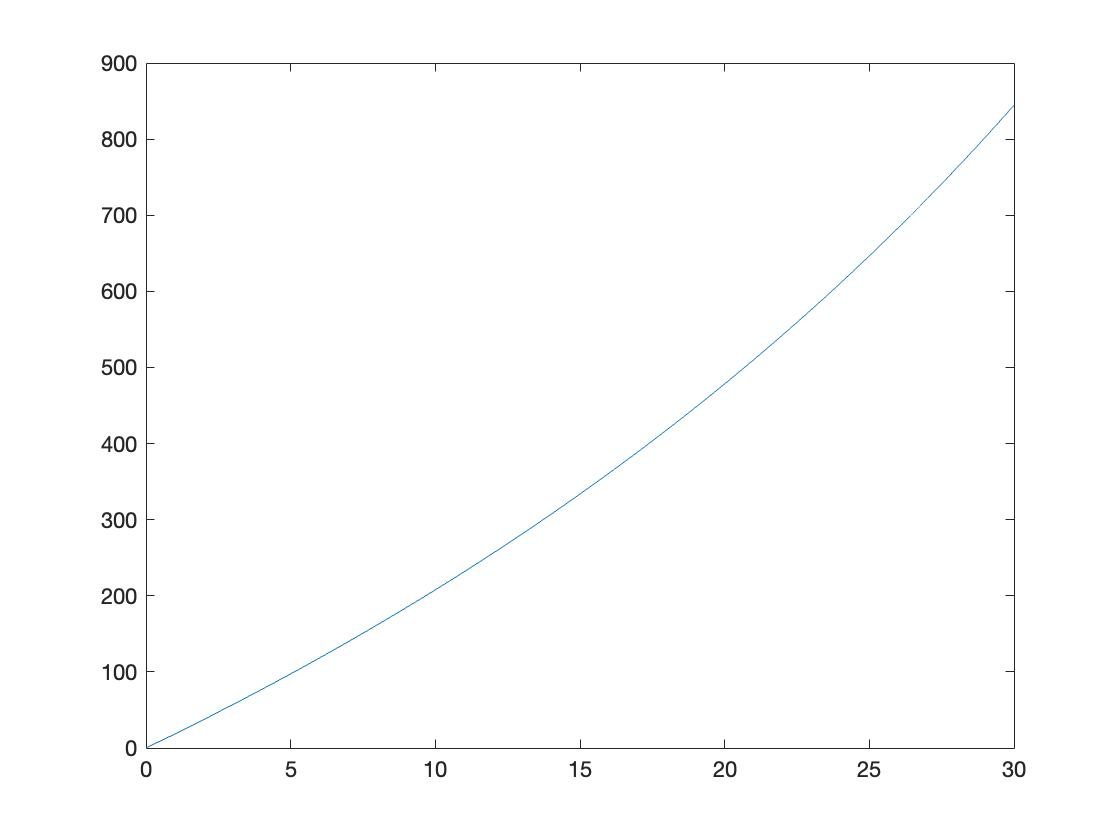
\includegraphics[width=12cm]{第五章作业/yuanhanshu.jpg}
    \caption{原函数}
\end{figure}
\begin{figure}[H]
    \centering
    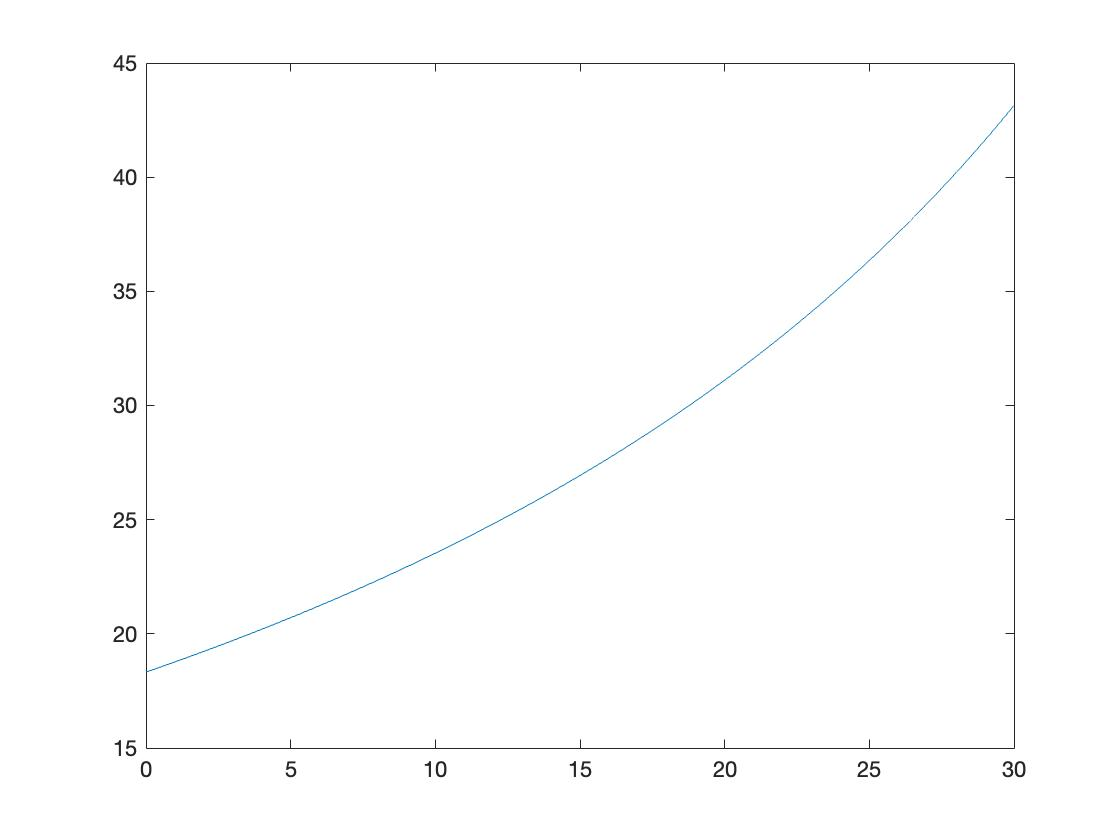
\includegraphics[width=12cm]{第五章作业/daohanshu.jpg}
    \caption{导函数}
\end{figure}
\par
对于第一问,使用Newton-Cotes积分中的梯形法、Simpson1/3法、Simpson3/8法、复合梯形法、
复合Simpson法、非等距积分,Romberg法,Guass法分别来估计计算积分值,并分析误差。
\par
对于第二问,使用差商近似法、插值型数值微分法来估计计算微分值。

\newpage
\tableofcontents

\newpage
\section{数值积分}
首先将$v$转换为函数文件并保存在v.m中:
\begin{lstlisting}
function out = v(t)
u=1800;m0=160000;q=2500;g=9.8;
out=u.*log(m0./(m0-q.*t))-g.*t;
end
\end{lstlisting}

\begin{figure}[H]
    \centering
    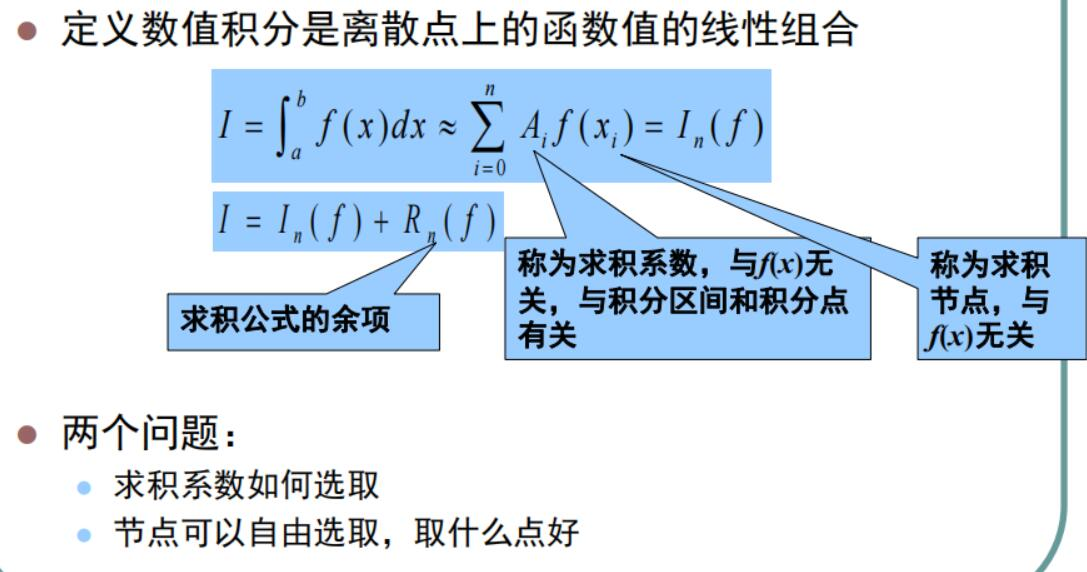
\includegraphics[width=14cm]{第五章作业/shuzhijifen.jpg}
\end{figure}
\begin{figure}[H]
    \centering
    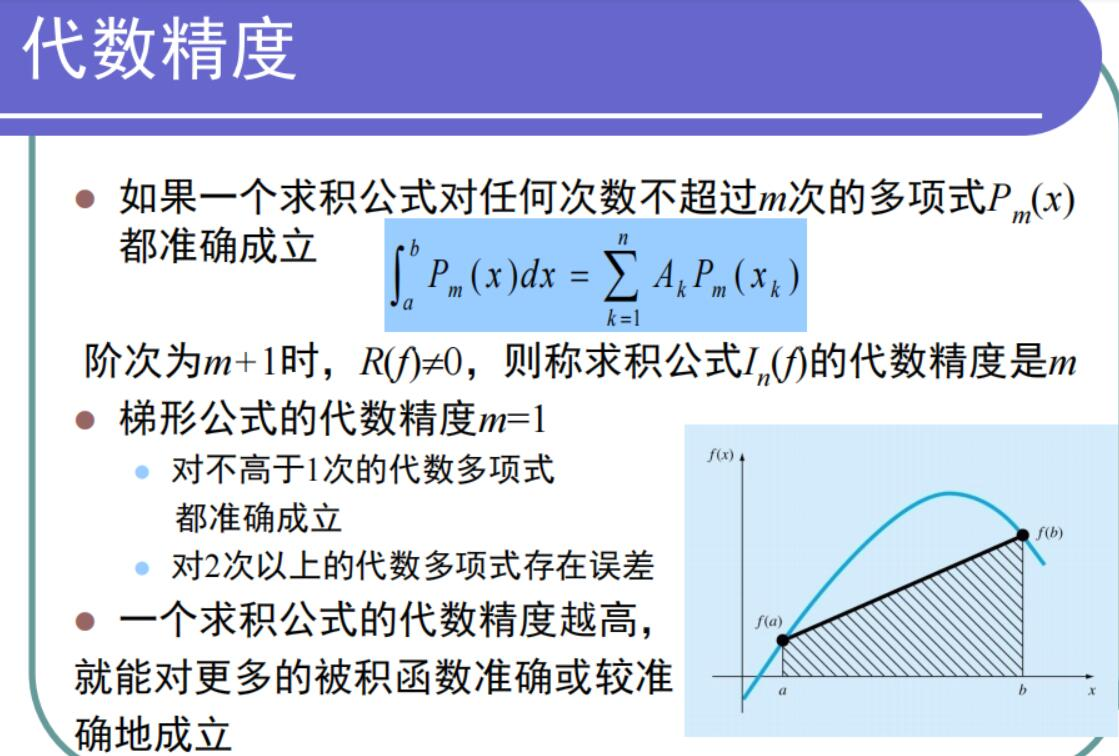
\includegraphics[width=14cm]{第五章作业/daishujingdu.jpg}
\end{figure}

\subsection{Newton-Cotes积分}
\begin{figure}[H]
    \centering
    \includegraphics[width=14cm]{第五章作业/n-c1.jpg}
\end{figure}
\begin{figure}[H]
    \centering
    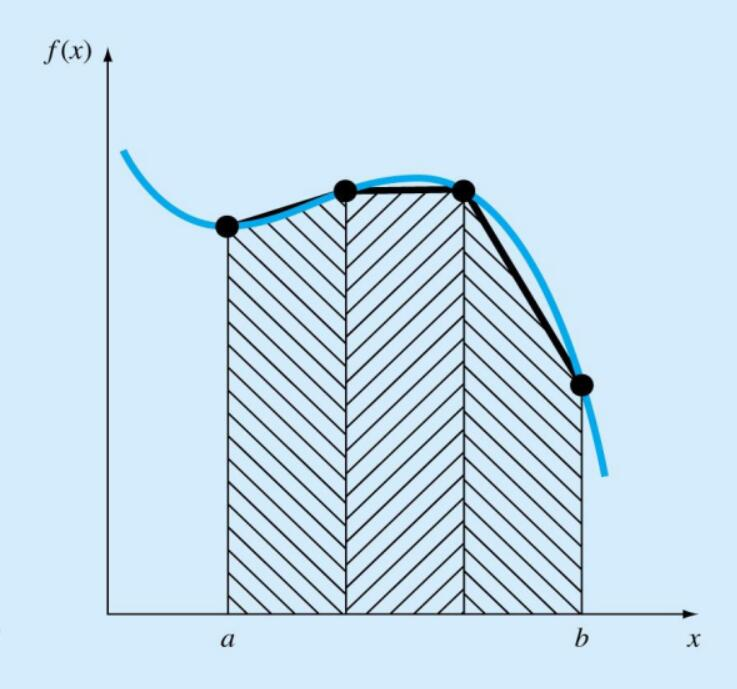
\includegraphics[width=7cm]{第五章作业/n-c2.jpg}
\end{figure}
\begin{figure}[H]
    \centering
    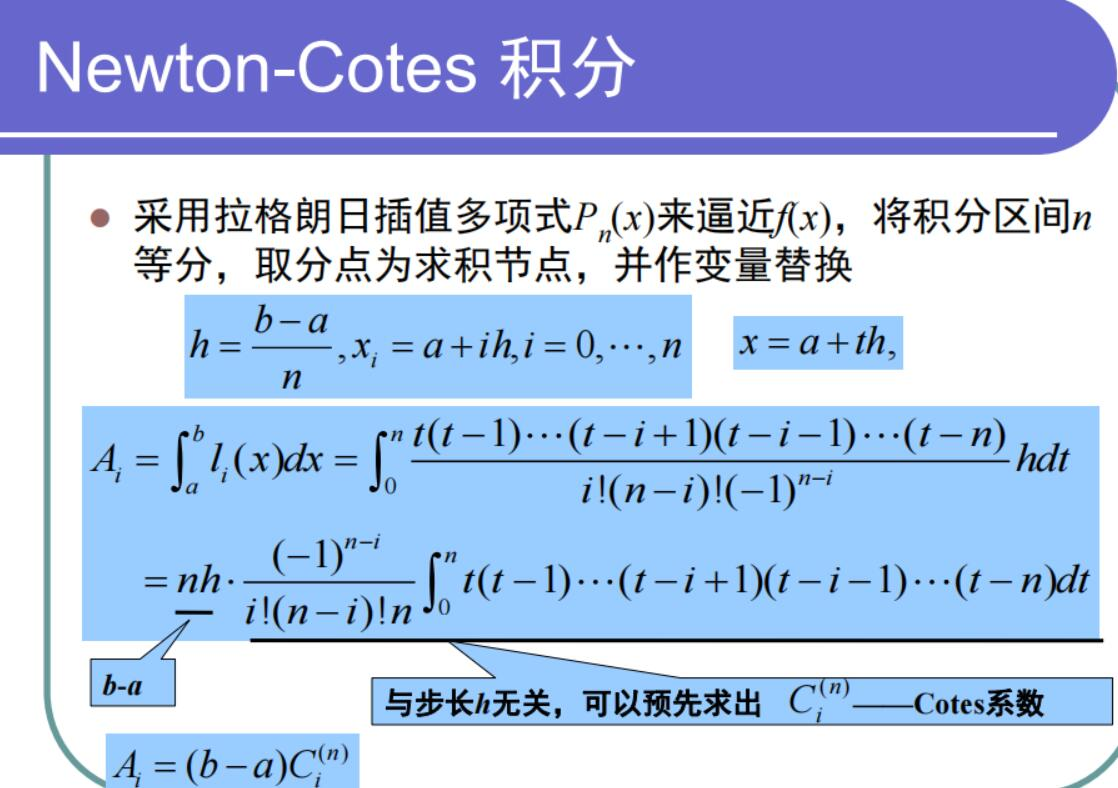
\includegraphics[width=12cm]{第五章作业/n-c3.jpg}
\end{figure}
\subsubsection{梯形公式}
\begin{figure}[H]
    \centering
    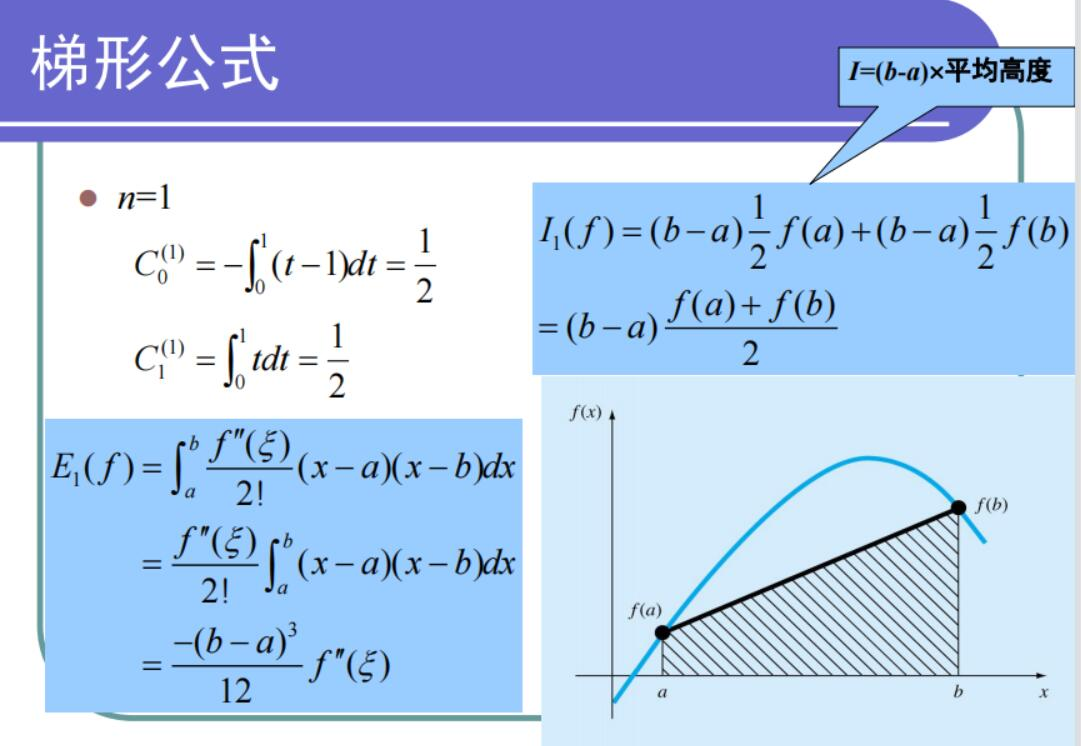
\includegraphics[width=14cm]{第五章作业/tixing.jpg}
\end{figure}
\begin{lstlisting}
%% Trapezoidal formula
clc,clear
I_real=10879.6194048972;
a=0;
b=30;
I=(b-a)*(v(a)+v(b))/2;
et=abs((I-I_real)/I_real);
e=abs(I-I_real);
\end{lstlisting}
\begin{table}[H]
    \centering
    \begin{tabular}{lll}
        \hline
        积分结果              & 与真值相对误差    & 与真值绝对误差        \\ \hline
        1.266810908607478e+04 & 0.164388993274208 & 1.788489681177583e+03 \\ \hline
    \end{tabular}
\end{table}
\par
估计误差:用原函数二阶导的积分平均值代替$f''(\zeta)$:
\begin{equation}
    f''(x)=\frac{\int_{0}^{30}(\frac{1800}{(64-t)^2})dt}{30-0}=0.8272
\end{equation}
\begin{equation}
    E_a=|-\frac{1}{12}*0.8272*30^3|=-1.8612e+03
\end{equation}
\par
可以看出,直接使用梯形公式的误差较大,且估计误差的绝对值略大于真实绝对误差的绝对值,误差估计有效。

\subsubsection{Simpson公式(Simpson1/3法则)}
\begin{figure}[H]
    \centering
    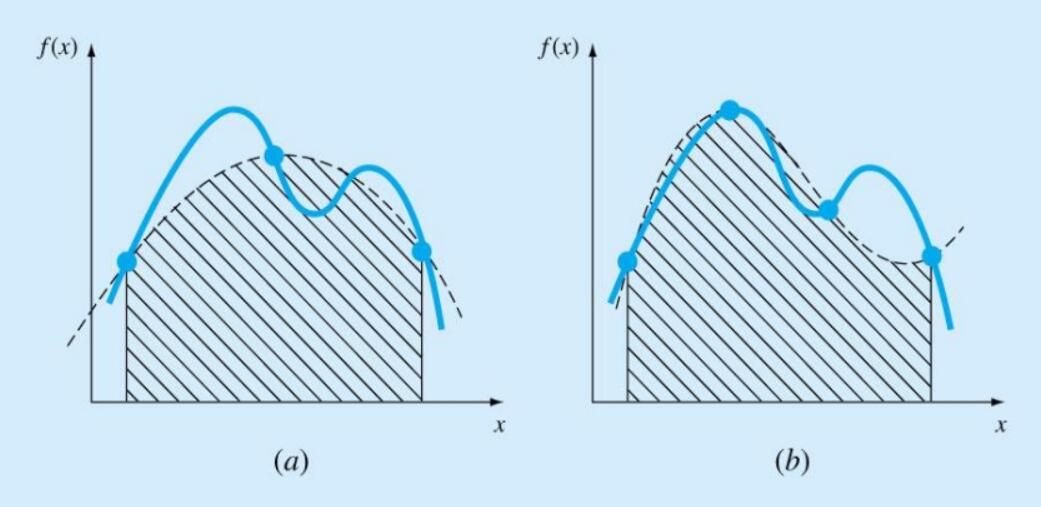
\includegraphics[width=14cm]{第五章作业/simpson1.jpg}
\end{figure}
\begin{figure}[H]
    \centering
    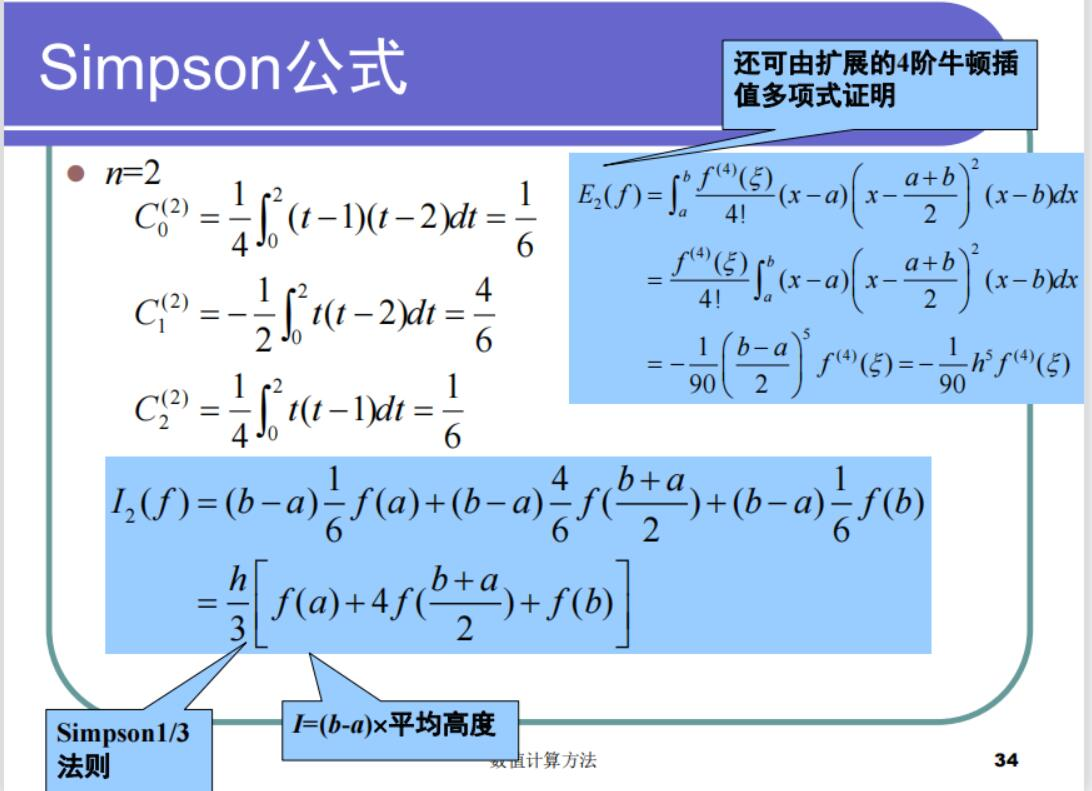
\includegraphics[width=14cm]{第五章作业/simpson2.jpg}
\end{figure}
\begin{lstlisting}
%% Simpson 1/3
clc,clear
I_real=10879.6194048972;
a=0;
b=30;
I=(b-a)/6*v(a)+(b-a)*4/6*v((a+b)/2)+(b-a)/6*v(b);
et=abs((I-I_real)/I_real);
e=abs(I-I_real);
\end{lstlisting}
\begin{table}[H]
    \centering
    \begin{tabular}{lll}
        \hline
        积分结果              & 与真值相对误差    & 与真值绝对误差     \\ \hline
        1.089696329765722e+04 & 0.001594163556145 & 17.343892760020026 \\ \hline
    \end{tabular}
\end{table}
\par
估计误差:用原函数四阶导的积分平均值代替$f^{(4)}(\zeta)$:
\begin{equation}
    f^{(4)}(x)=\frac{\int_{0}^{30}(\frac{10800}{(64-t)^4})dt}{30-0}=0.0025953607
\end{equation}
\begin{equation}
    E_a=|-\frac{1}{90}*0.0025953607*15^5|=21.8983
\end{equation}
\par
可以看出,误差比直接使用梯形公式的小了一些,且估计误差的绝对值略大于真实绝对误差的绝对值,误差估计有效。


\subsubsection{Simpson3/8法则}
\begin{figure}[H]
    \centering
    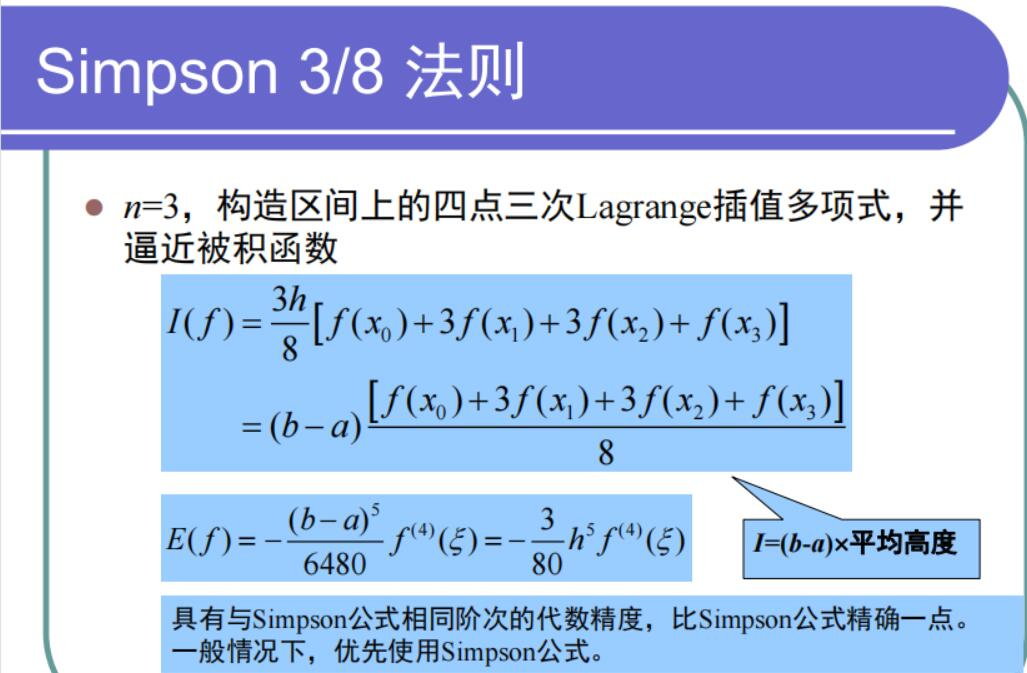
\includegraphics[width=14cm]{第五章作业/simpson3.jpg}
\end{figure}
\begin{lstlisting}
%% Simpson 3/8
clc,clear
I_real=10879.6194048972;
a=0;
b=30;
x0=0;x1=10;x2=20;x3=30;
I=(b-a)*(v(x0)+3*v(x1)+3*v(x2)+v(x3))/8;
et=abs((I-I_real)/I_real);
e=abs(I-I_real);
\end{lstlisting}
\begin{table}[H]
    \centering
    \begin{tabular}{lll}
        \hline
        积分结果              & 与真值相对误差        & 与真值绝对误差    \\ \hline
        1.088752511781406e+04 & 7.266534446327055e-04 & 7.905712916861376 \\ \hline
    \end{tabular}
\end{table}
\par
估计误差:用原函数四阶导的积分平均值代替$f^{(4)}(\zeta)$:
\begin{equation}
    f^{(4)}(x)=\frac{\int_{0}^{30}(\frac{10800}{(64-t)^4})dt}{30-0}=0.0025953607
\end{equation}
\begin{equation}
    E_a=|-\frac{3}{80}*0.0025953607*10^5|=9.7326
\end{equation}
\par
可以看出,Simpson3/8法则闭Simpson1/3法则的误差又的小了一些,且估计误差的绝对值略大于真实绝对误差的绝对值,误差估计有效。


\subsubsection{复合梯形公式}
\begin{figure}[H]
    \centering
    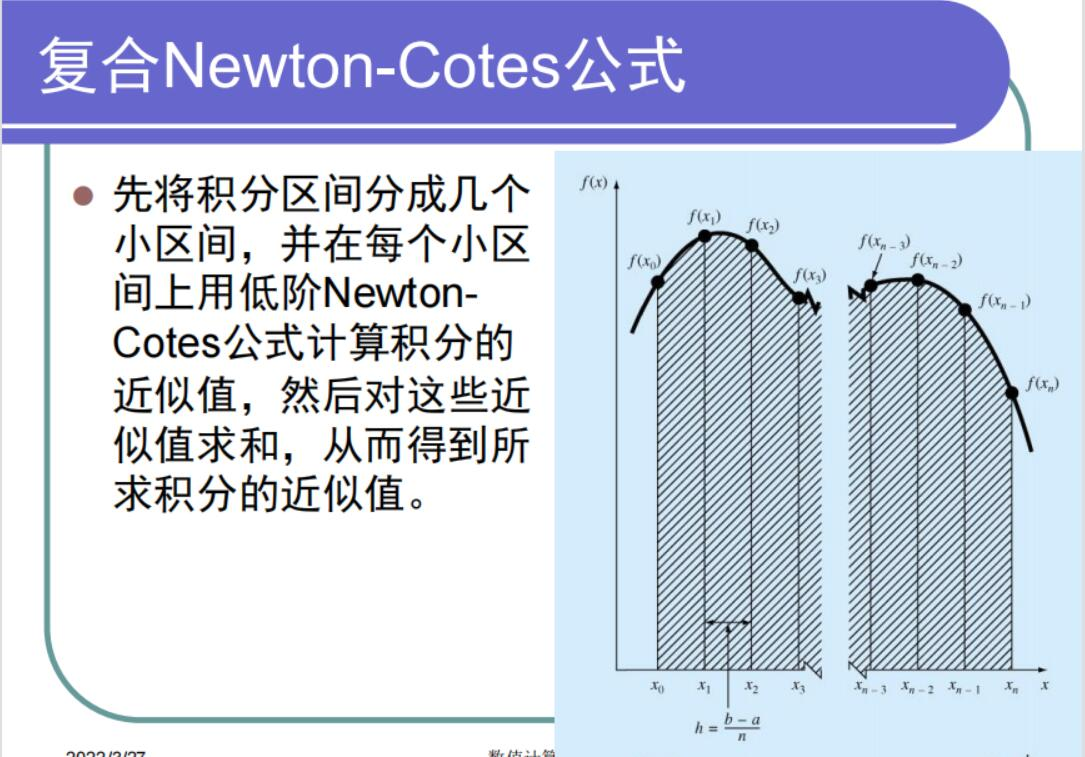
\includegraphics[width=14cm]{第五章作业/n-c4.jpg}
\end{figure}
\begin{figure}[H]
    \centering
    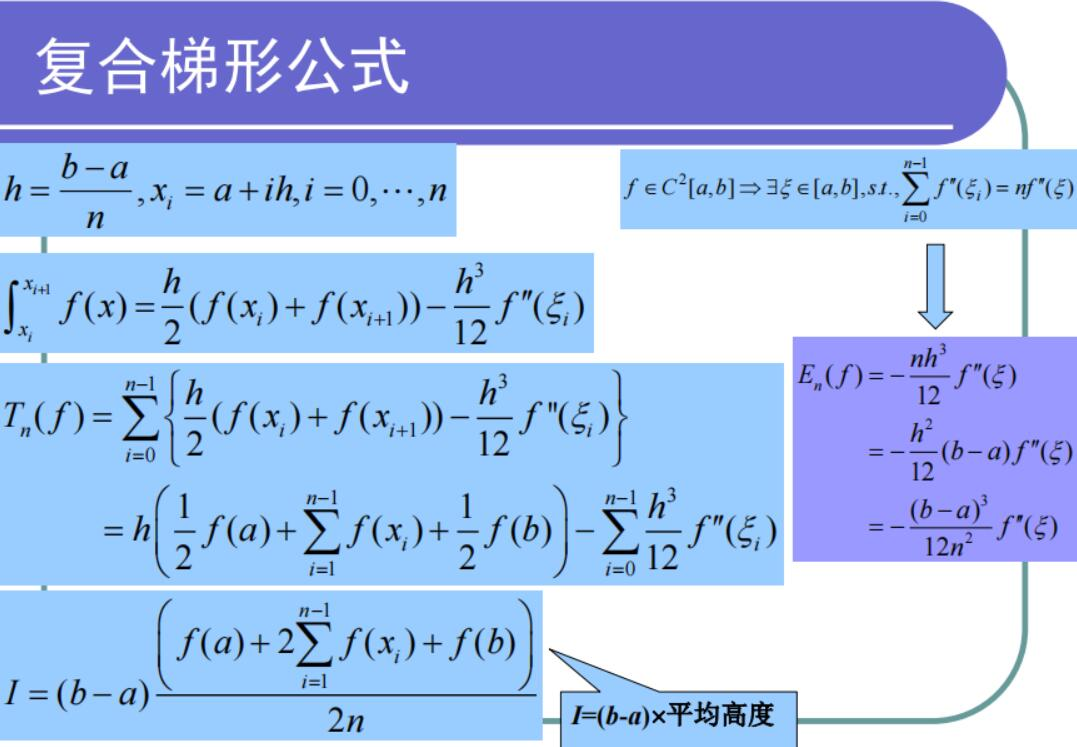
\includegraphics[width=14cm]{第五章作业/futi.jpg}
\end{figure}
\begin{lstlisting}
%% combined trapz
clc,clear
I_real=10879.6194048972;
a=0;
b=30;
n=100;
x=linspace(a,b,n+1); 
h=(b-a)/n;
I=(v(x(1))+v(x(n+1)))/2+sum(v(x(2:n))); 
I=I*h;
et=abs((I-I_real)/I_real);
e=abs(I-I_real);
\end{lstlisting}
\par
复合梯形法的误差可以被控制。在计算中,由于$f''(x)$是一个下凸函数,因此用原函数二阶导的积分
平均值代替$f''(\zeta)$来估计误差是可以保证不等号方向的。
\begin{equation}
    f''(x)=\frac{\int_{0}^{30}(\frac{1800}{(64-t)^2})dt}{30-0}=0.8272
\end{equation}
\par
若要使绝对误差限$E=5e-05$,可以由公式算出:
\begin{equation}
    n\geq \sqrt{\frac{30^3}{12}*\frac{f''(\zeta)}{E}}=6101.15
\end{equation}
\par
因此,理论上$n$大于等于6102即可。
\begin{table}[H]
    \centering
    \begin{tabular}{llll}
        \hline
        $n$   & 积分结果              & 与真值相对误差        & 与真值绝对误差        \\ \hline
        1     & 1.266810908607478e+04 & 0.164388993274208     & 1.788489681177583e+03 \\
        100   & 1.087980552534478e+04 & 1.710725721633231e-05 & 0.186120447575377     \\
        1000  & 1.087962126611031e+04 & 1.710733657619924e-07 & 0.001861213109805     \\
        5000  & 1.087961947934569e+04 & 6.842931433761493e-09 & 7.444848961313255e-05 \\
        6101  & 1.087961945489993e+04 & 4.596000174000550e-09 & 5.000273267796729e-05 \\
        6102  & 1.087961945488355e+04 & 4.594494606666866e-09 & 4.998635267838836e-05 \\
        10000 & 1.087961942350929e+04 & 1.710730266958566e-09 & 1.861209420894738e-05 \\
        \hline
    \end{tabular}
\end{table}
经过实践验证,我惊讶地发现理论结果与实际结果恰好吻合,正好是在$n$=6102处绝对误差降到5e-05以下,
因此用原函数二阶导的积分平均值代替$f''(\zeta)$来估计误差非常的有效。

\subsubsection{复合Simpson公式}
\begin{figure}[H]
    \centering
    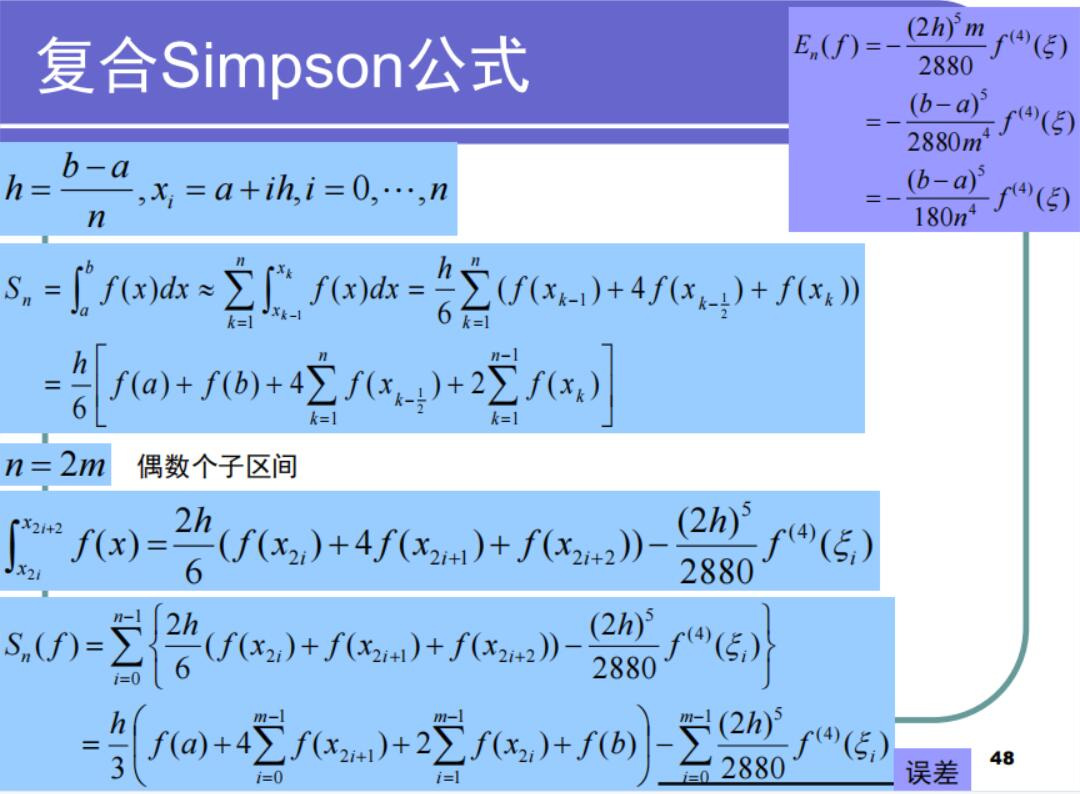
\includegraphics[width=14cm]{第五章作业/fusimpson.jpg}
\end{figure}
\begin{lstlisting}
%% combined simpson
clc,clear
I_real=10879.6194048972;
a=0;
b=30;
n=100;
m=round(n/2);
x=linspace(a,b,2*m+1);
h=(b-a)/2/m;
I=(v(a)+v(b)+4*sum(v(x(2:2:2*m)))+2*sum(v(x(3:2:2*m-1)))); 
I=I*h/3;
et=abs((I-I_real)/I_real);
e=abs(I-I_real);
\end{lstlisting}
\begin{table}[H]
    \centering
    \begin{tabular}{lll}
        \hline
        积分结果              & 与真值相对误差        & 与真值绝对误差        \\ \hline
        1.087961940840046e+04 & 3.220018132555801e-10 & 3.503257175907493e-06 \\ \hline
    \end{tabular}
\end{table}
\par
复合Simpson的误差可以被控制。在计算中,由于$f^{(4)}(x)$是一个下凸函数,因此用原函数二阶导的积分
平均值代替$f^{(4)}(\zeta)$来估计误差是可以保证不等号方向的。
\begin{equation}
    f^{(4)}(x)=\frac{\int_{0}^{30}(\frac{10800}{(64-t)^4})dt}{30-0}=0.0025953607
\end{equation}
\begin{equation}
    n\geq \sqrt[4]{\frac{30^5}{180}*\frac{f^{(4)}(\zeta)}{E}}=51.45
\end{equation}
因此,理论上$n$大于等于52即可(注意这里的$n$必须是偶数)。
\begin{table}[H]
    \centering
    \begin{tabular}{llll}
        \hline
        $n$ & 积分结果              & 与真值相对误差        & 与真值绝对误差        \\ \hline
        2   & 1.089696329765722e+04 & 0.001594163556145     & 17.343892760020026    \\
        10  & 1.087965401388441e+04 & 3.181084367287731e-06 & 0.034608987210959     \\
        50  & 1.087961946092888e+04 & 5.150150772952511e-09 & 5.603168028756045e-05 \\
        52  & 1.087961945279512e+04 & 4.402536192757309e-09 & 4.789791819348466e-05 \\
        100 & 1.087961940840046e+04 & 3.220018132555801e-10 & 3.503257175907493e-06 \\
        \hline
    \end{tabular}
\end{table}
经过实践验证,理论结果与实际结果也是恰好吻合,正好是在$n$=52处绝对误差降到5e-05以下,
因此用原函数四阶导的积分平均值代替$f^{(4)}(\zeta)$来估计误差非常的有效。

\subsubsection{非等距积分(步长自适应)}
\begin{figure}[H]
    \centering
    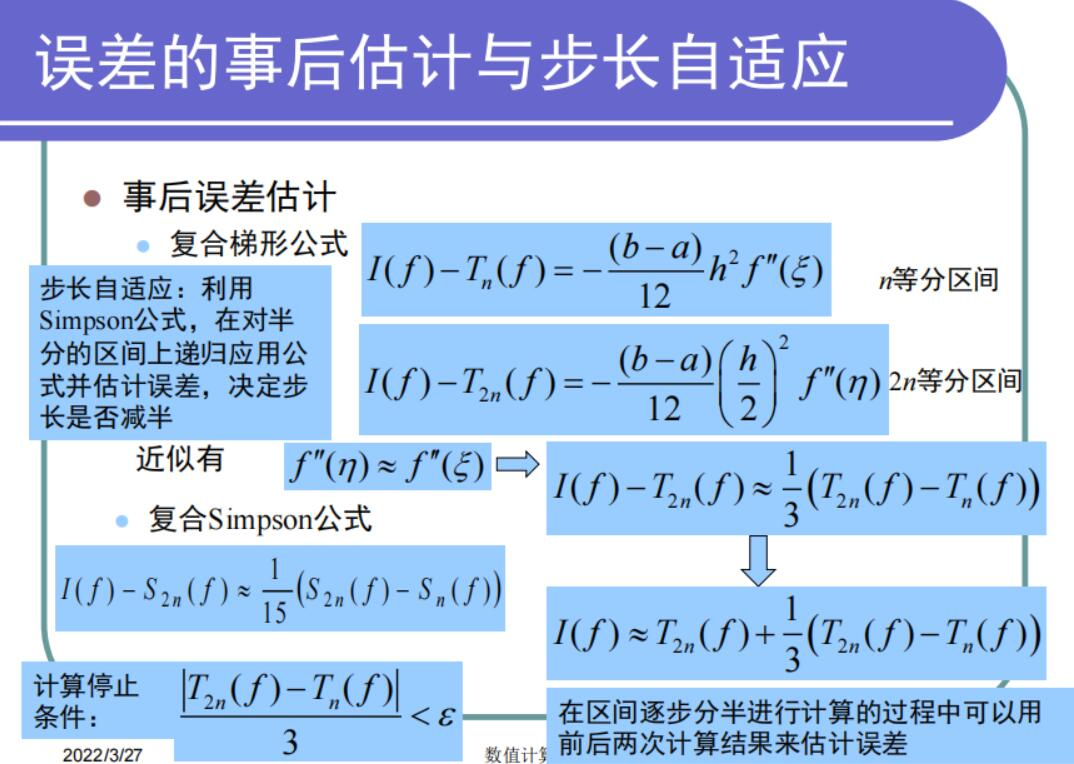
\includegraphics[width=14cm]{第五章作业/feidengju.jpg}
\end{figure}
\begin{lstlisting}
%% Step size adaptation
clc,clear
I_real=10879.6194048972;
tol=5e-5;
a=0;
b=30;
c=(a+b)/2;
fa=v(a);fb=v(b);fc=v(c);
I=quadstep(a,b,tol,fa,fc,fb);
et=abs((I-I_real)/I_real);
e=abs(I-I_real);

function q=quadstep(a,b,tol,fa,fc,fb)
% Recursive subfunction used by quadadapt.
h=b-a;c=(a+b)/2;
fd=v((a+c)/2);fe=v((c+b)/2);
q1=h/6*(fa+4*fc+fb);
q2=h/12*(fa+4*fd+2*fc+4*fe+fb);
% 满足精度,跳出函数
if abs(q2-q1)<=tol
    q=q2+(q2-q1)/15;
% 不满足精度,继续迭代递归
else
    qa=quadstep(a,c,tol,fa,fd,fc);
    qb=quadstep(c,b,tol,fc,fe,fb);
    q=qa+qb;
end
end
\end{lstlisting}
\begin{table}[H]
    \centering
    \begin{tabular}{lll}
        \hline
        积分结果              & 与真值相对误差        & 与真值绝对误差        \\ \hline
        1.087961940491261e+04 & 1.416788182747394e-12 & 1.541411620564759e-08 \\ \hline
    \end{tabular}
\end{table}
\par
从运行结果中可以看出,实际与真值绝对误差在给定误差限以下,步长自适应的非等距积分可以完成误差控制。

\subsection{Romberg积分}
\begin{figure}[H]
    \centering
    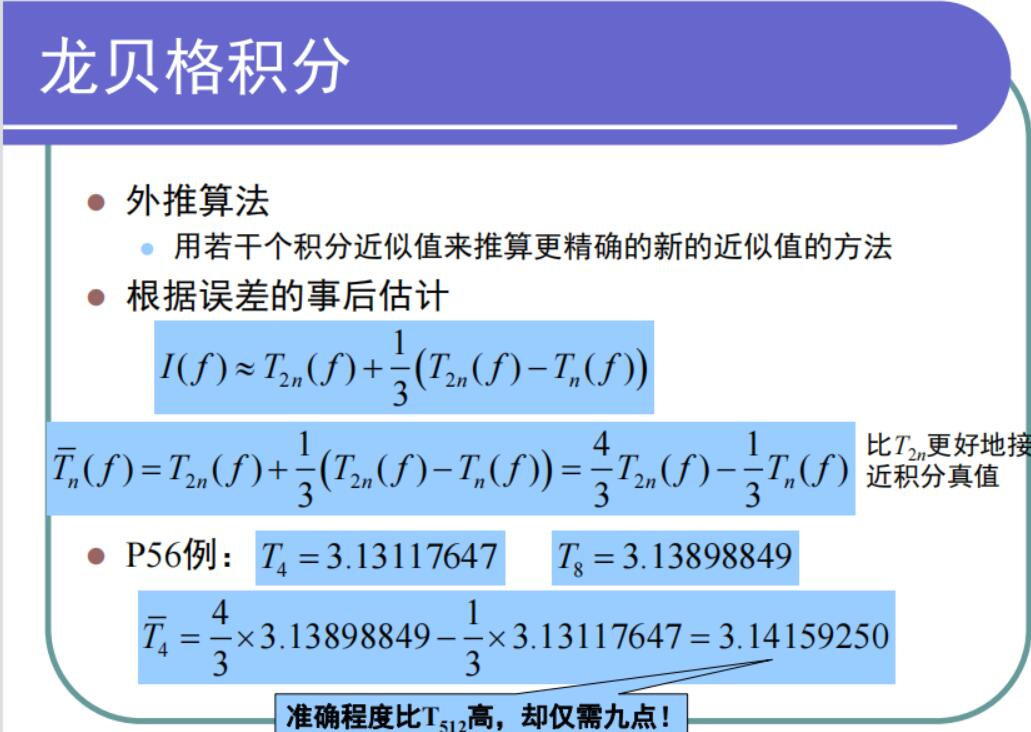
\includegraphics[width=14cm]{第五章作业/rb1.jpg}
\end{figure}
\begin{figure}[H]
    \centering
    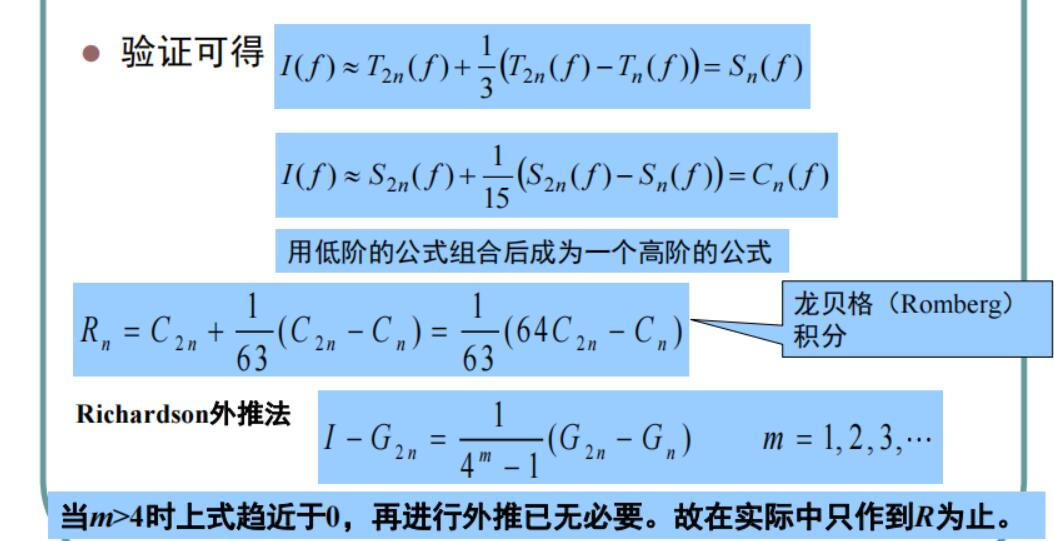
\includegraphics[width=14cm]{第五章作业/rb2.jpg}
\end{figure}
\begin{figure}[H]
    \centering
    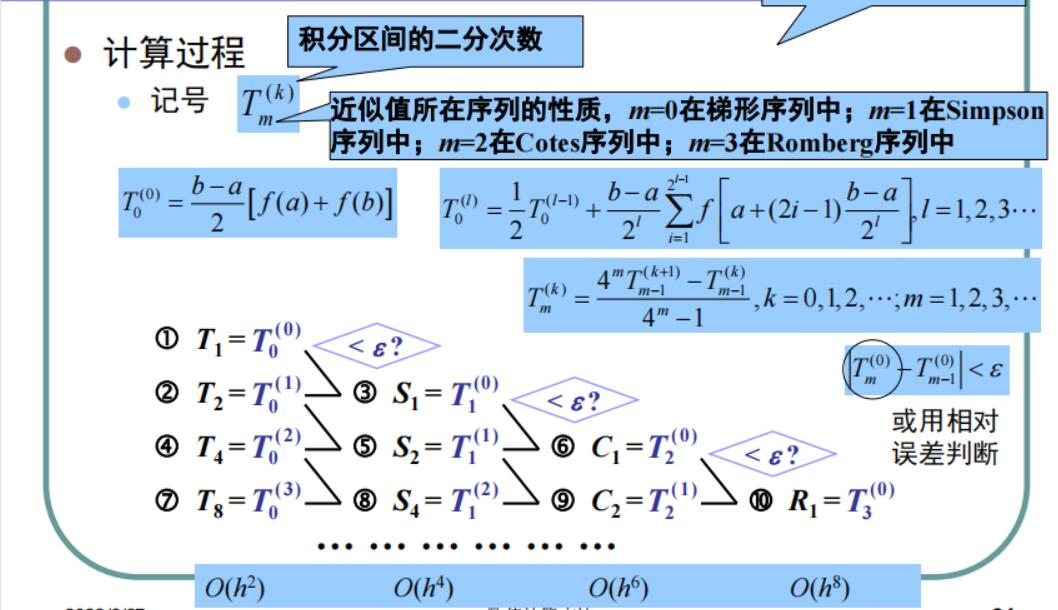
\includegraphics[width=14cm]{第五章作业/rb3.jpg}
\end{figure}
\subsubsection{普通Romberg积分}
\begin{lstlisting}
%% Romberg
clc,clear
I_real=10879.6194048972;
a=0;
b=30;
j=0;t=5;% 迭代次数
M=[];
h=(b-a)/2^j;
M(1,1)=h*(v(a)+v(b))/2;
for j=2:t
    h=h/2;
    M(j,1)=0.5*M(j-1,1)+h*sum(v(a+h*(1:2:2^(j-1)))); 
end
for k=2:t
    M(k:t,k)=M(k:t,k-1)+(M(k:t,k-1)-M(k-1:t-1,k-1))/(4^(k-1)-1); % 龙贝格公式
end
et=abs((M(5,5)-I_real)/I_real);
e=abs(M(5,5)-I_real);
\end{lstlisting}
\begin{table}[H]
    \centering
    \begin{tabular}{lll}
        \hline
        积分结果              & 与真值相对误差        & 与真值绝对误差        \\ \hline
        1.087961940894866e+04 & 3.723895823567930e-10 & 4.051456926390529e-06 \\ \hline
    \end{tabular}
\end{table}
然而,传统的龙贝格积分难以控制误差,因此有下面改进后的龙贝格积分。

\subsubsection{改进的Romberg积分}
\begin{lstlisting}
%% Romberg step adaptation
clc,clear
I_real=10879.6194048972;
a=0;
b=30;
tol=5e-10;% 给定误差
j=1;
M=[];
h=b-a;
M(1)=h*(v(a)+v(b))/2;
M(2)=inf;
while (abs(M(1)-M(2))>tol)% 估计相对误差
    j=j+1;
    h=h/2;
    M(j)=0.5*M(j-1)+h*sum(v(a+h*(1:2:2^(j-1))));
    for k=j-1:-1:1
        M(k)=M(k+1)+(M(k+1)-M(k))/(4^(j-k)-1); 
    end
end
I=M(1);
et=abs((M(1)-I_real)/I_real);
e=abs(M(1)-I_real);
\end{lstlisting}
\begin{table}[H]
    \centering
    \begin{tabular}{lll}
        \hline
        积分结果              & 与真值相对误差        & 与真值绝对误差        \\ \hline
        1.087961940489716e+04 & 3.511039867559036e-15 & 3.819877747446299e-11 \\ \hline
    \end{tabular}
\end{table}
\par
可以看出,利用改进后的龙贝格公式,成功将实际绝对误差降到了给定误差限以下。

\subsection{Guass求积公式}
\begin{figure}[H]
    \centering
    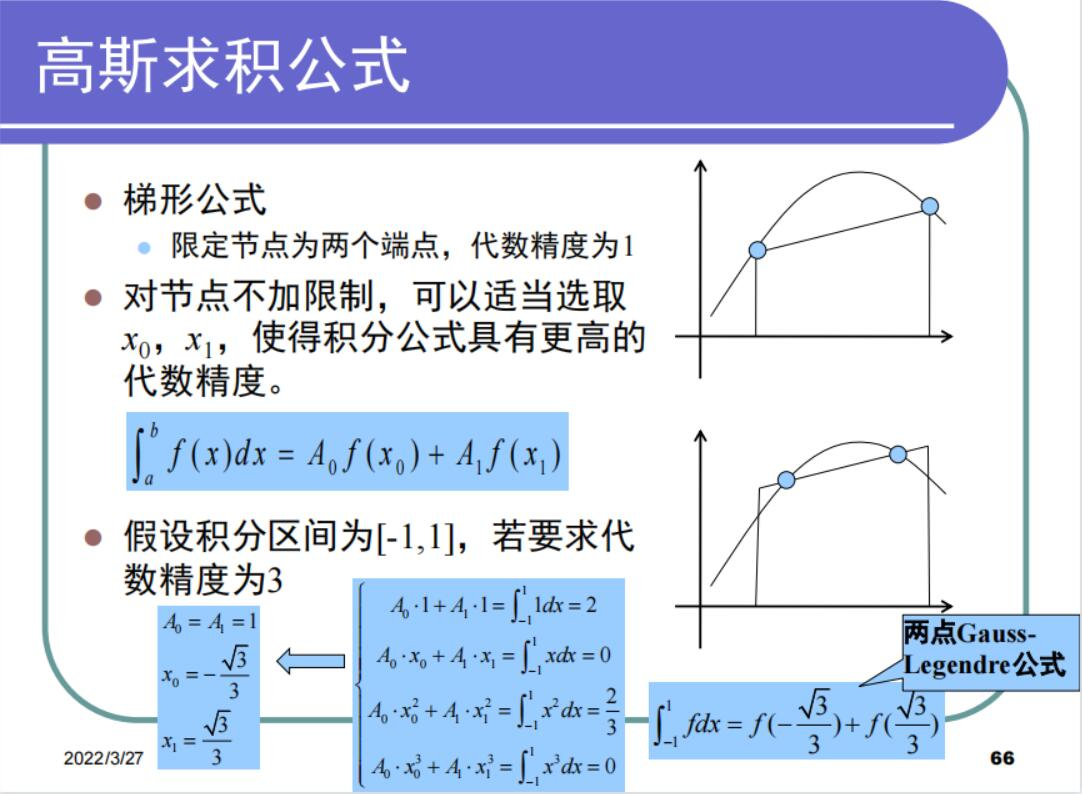
\includegraphics[width=14cm]{第五章作业/gs1.jpg}
\end{figure}
\begin{figure}[H]
    \centering
    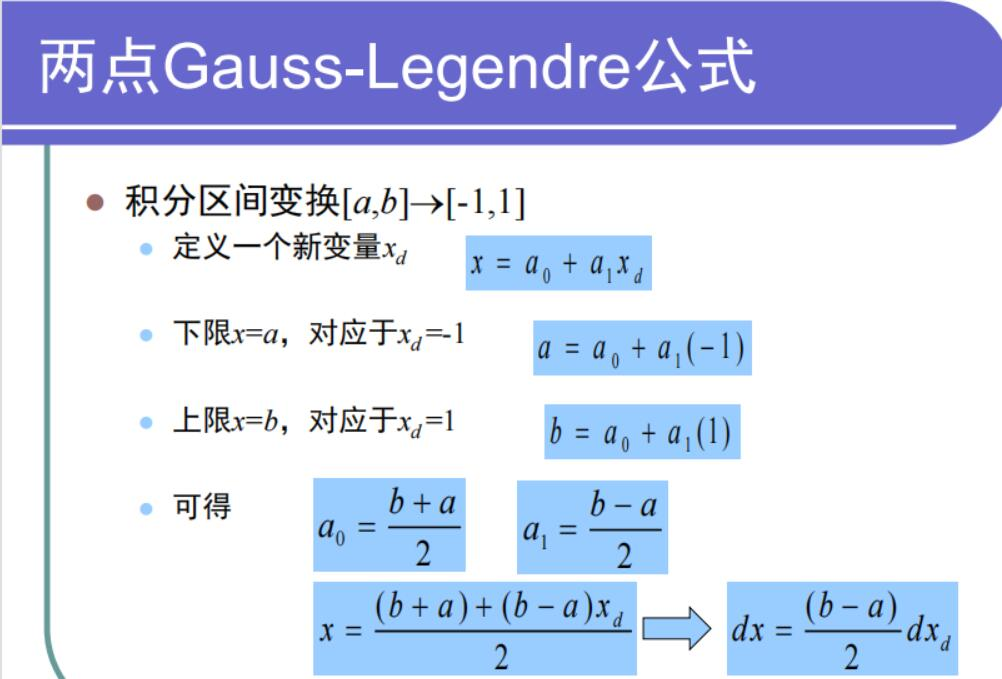
\includegraphics[width=14cm]{第五章作业/gs2.jpg}
\end{figure}
\begin{figure}[H]
    \centering
    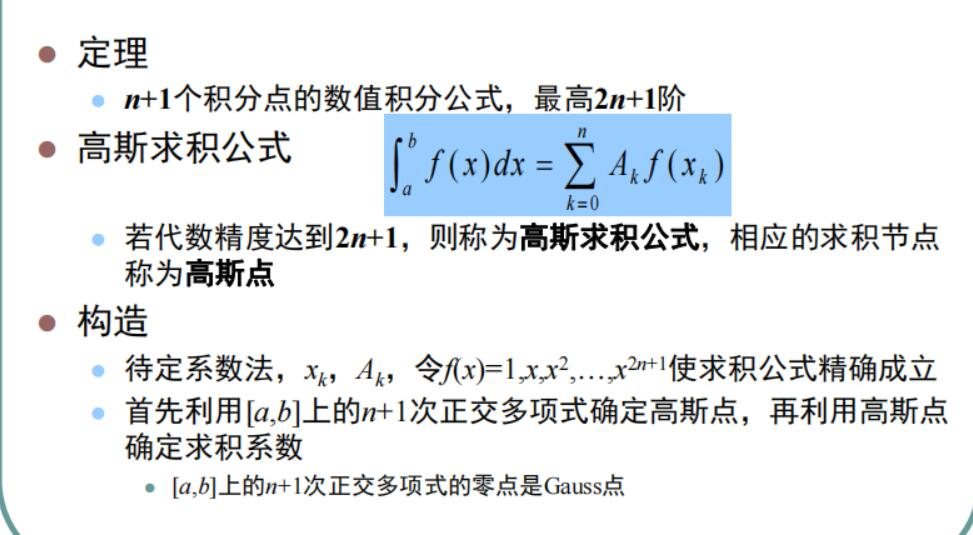
\includegraphics[width=14cm]{第五章作业/gs3.jpg}
\end{figure}
\subsubsection{单段Guass求积}
\begin{lstlisting}
%% Guass
clc,clear
I_real=10879.6194048972;
a=0;
b=30;
a0=(a+b)/2;
a1=(b-a)/2;
% three points
I=5/9*v_(-sqrt(15)/5,a0,a1)+8/9*v_(0,a0,a1)+5/9*v_(sqrt(15)/5,a0,a1);
et=abs((I-I_real)/I_real);
e=abs(I-I_real);

function out=v_(t,a0,a1)
out=v(a0+a1*t)*a1;
end
\end{lstlisting}
\begin{table}[H]
    \centering
    \begin{tabular}{lll}
        \hline
        积分结果              & 与真值相对误差        & 与真值绝对误差    \\ \hline
        1.087942772294797e+04 & 1.761844253008763e-05 & 0.191681949234408 \\ \hline
    \end{tabular}
\end{table}
\par
同样是取3个点,相比于Simpson1/3法则的误差17.343892760020026,Simpson3/8法则的误差
7.905712916861376,可以看出使用高斯求积公式可以将误差大大减小。

\subsubsection{复合Guass求积}
利用Guass求积公式时,较多采用复合求积的方法,将积分区间分成$m$个等长的小区间,
在每个小区间上使用同一低阶Gauss求积公式算出积分的近似值,再相加。
\begin{lstlisting}
%% combined guass
clc,clear
I_real=10879.6194048972;
a=0;
I=0;
n=100;% 分割段数
for b=30/n:30/n:30
    a=b-30/n;
    a0=(a+b)/2;
    a1=(b-a)/2;
    % three points
    I=I+5/9*v_(-sqrt(15)/5,a0,a1)+8/9*v_(0,a0,a1)+5/9*v_(sqrt(15)/5,a0,a1);
end
et=abs((I-I_real)/I_real);
e=abs(I-I_real);

% 自变量转换
function out=v_(t,a0,a1)
out=v(a0+a1*t)*a1;
end
\end{lstlisting}
\begin{table}[H]
    \centering
    \begin{tabular}{lll}
        \hline
        积分结果              & 与真值相对误差        & 与真值绝对误差        \\ \hline
        1.087961940489718e+04 & 1.671923746456684e-15 & 1.818989403545857e-11 \\ \hline
    \end{tabular}
\end{table}
同样相较Simpson公式,相同采样条件下误差大大减小。

\subsection{数值积分总结}


\section{数值微分}
\subsection{差商近似}
\subsubsection{有限差商近似}
\begin{figure}[H]
    \centering
    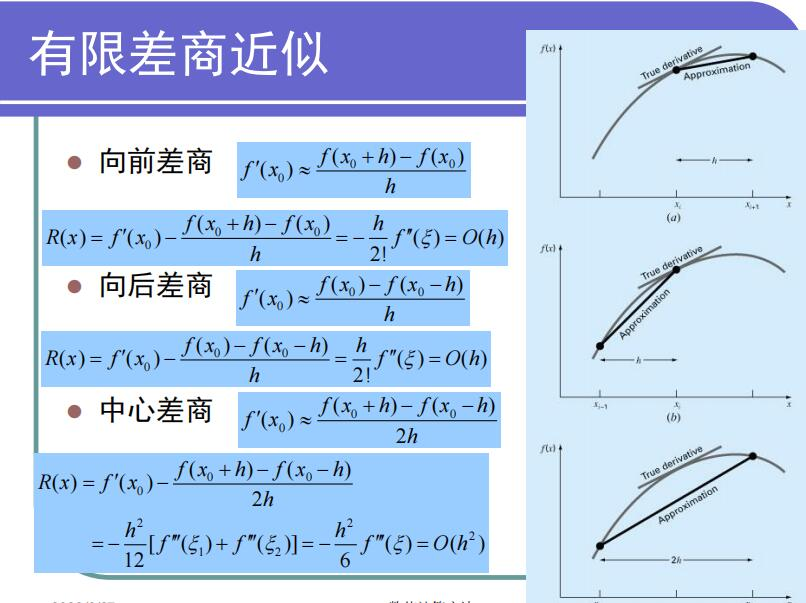
\includegraphics[width=14cm]{第五章作业/chashang.jpg}
\end{figure}
\begin{lstlisting}
%% Difference quotient approximation
clc,clear
a=0;
b=30;
step=1e-4;
x=a:step:b;
dv=1800./(64-x)-9.8;
subplot(4,1,1);
plot(x,dv,'r');% 精确值
title('精确值');
h=1e-4;
for i=1:b/step+1
    dv1(i)=(v(x(i)+h)-v(x(i)))/h;
end
subplot(4,1,2);
plot(x,dv1,'b');% 向前差商
title('向前差商');
for i=1:b/step+1
    dv2(i)=(v(x(i))-v(x(i)-h))/h;
end
subplot(4,1,3);
plot(x,dv2,'b');% 向后差商
title('向后差商');
for i=1:b/step+1
    dv3(i)=(v(x(i)+h)-v(x(i)-h))/2/h;
end
subplot(4,1,4);
plot(x,dv3,'b');% 中心差商
title('中心差商');
\end{lstlisting}
\begin{figure}[H]
    \centering
    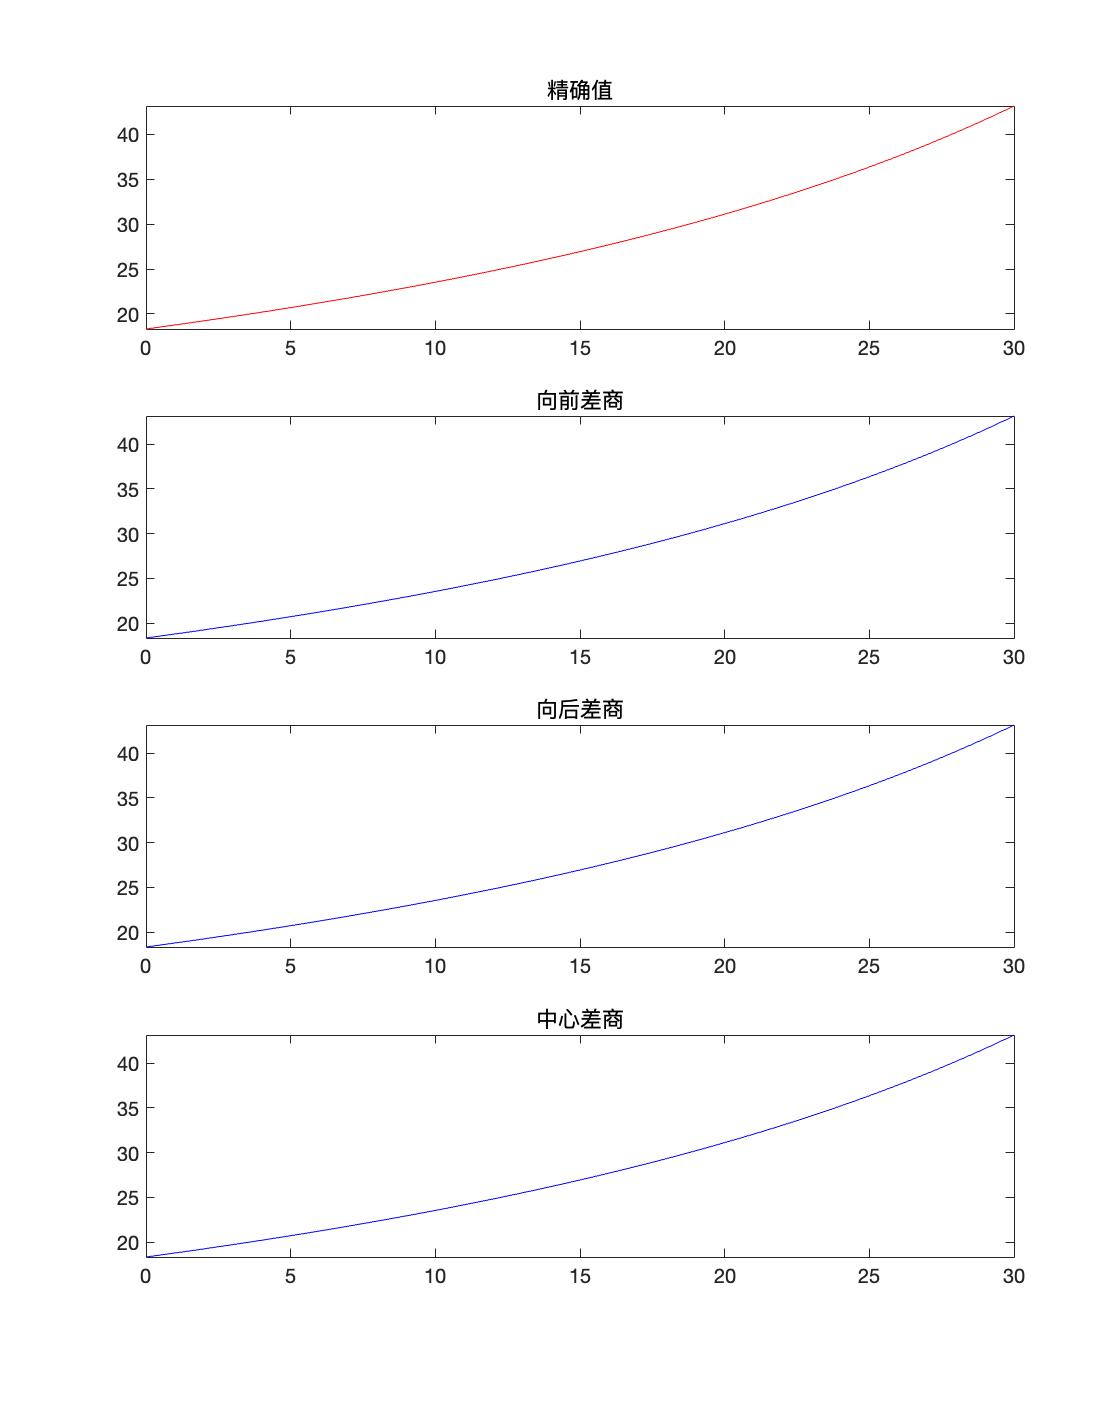
\includegraphics[width=10.5cm]{第五章作业/youxianchashang.jpg}
    \caption{有限差商近似(步长1e-4)}
\end{figure}
\begin{figure}[H]
    \centering
    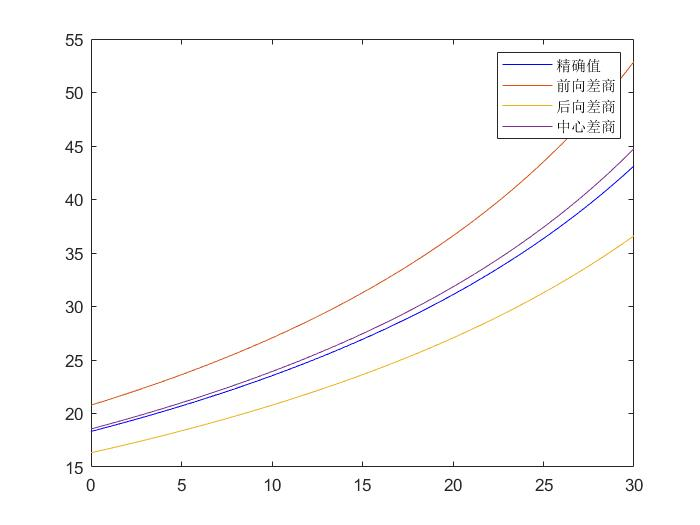
\includegraphics[width=10.5cm]{第五章作业/chashang10.jpg}
    \caption{有限差商近似(步长10)}
\end{figure}

\subsubsection{高精度微分公式}
\begin{figure}[H]
    \centering
    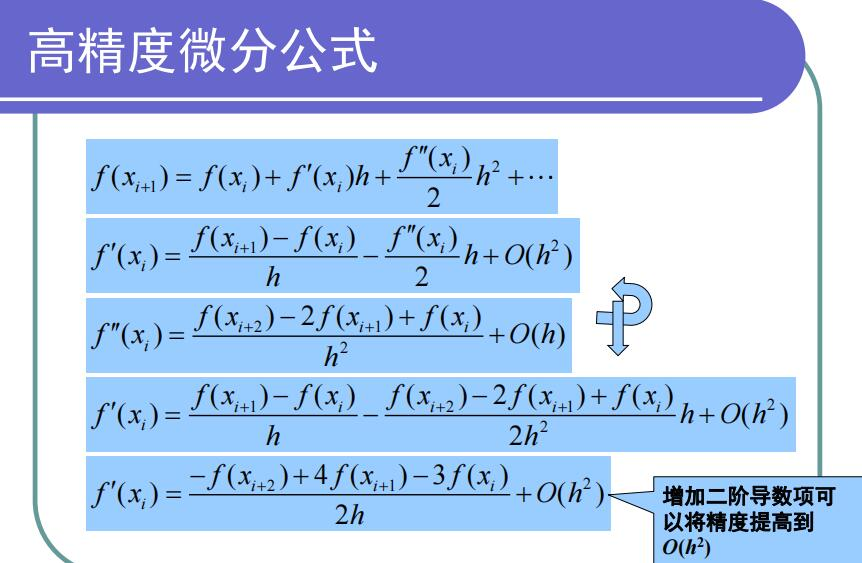
\includegraphics[width=14cm]{第五章作业/gjd.jpg}
\end{figure}
\begin{lstlisting}
%% High precision difference quotient
clc,clear
a=0;
b=30;
step=1e-4;
x=a:step:b;
dv=1800./(64-x)-9.8;
subplot(4,1,1);
plot(x,dv,'r');% 精确值
title('精确值');
h=1e-4;
for i=1:b/step+1
    dv1(i)=(-v(x(i)+2*h)+4*v(x(i)+h)-3*v(x(i)))/2/h;
end
subplot(4,1,2);
plot(x,dv1,'b');% 前向差商
title('前向差商');
for i=1:b/step+1
    dv2(i)=(3*v(x(i))-4*v(x(i)-h)+v(x(i)-2*h))/2/h;
end
subplot(4,1,3);
plot(x,dv2,'b');% 后向差商
title('后向差商');
for i=1:b/step+1
    dv3(i)=(-v(x(i)+2*h)+8*v(x(i)+h)-8*v(x(i)-h)+v(x(i)-2*h))/2/h;
end
subplot(4,1,4);
plot(x,dv3,'b');% 中心差商
title('中心差商');
\end{lstlisting}

\begin{figure}[H]
    \centering
    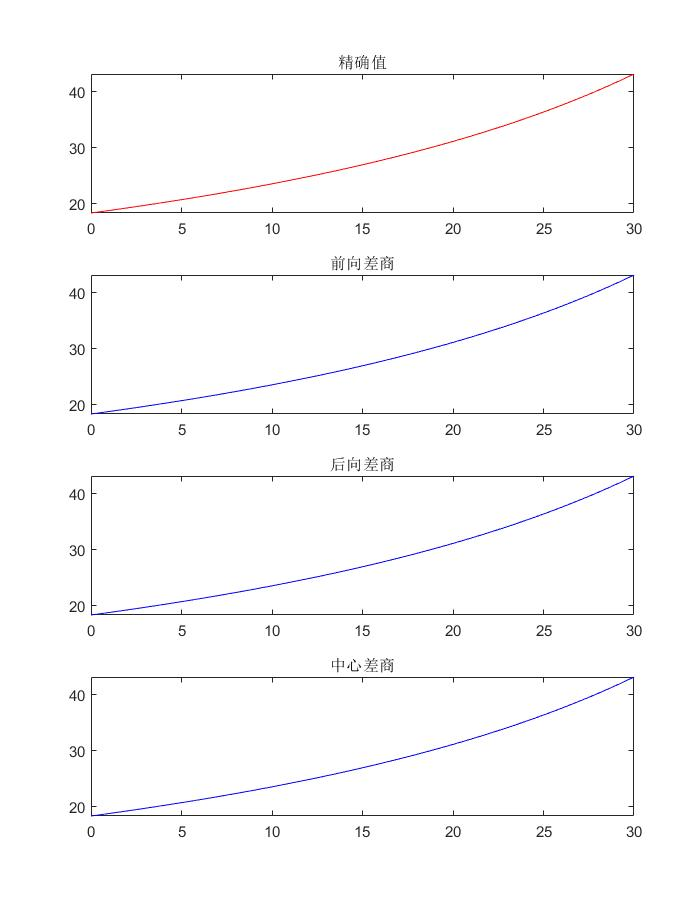
\includegraphics[width=10.5cm]{第五章作业/gaojingdu.jpg}
    \caption{高精度微分公式(步长1e-4)}
\end{figure}
\begin{figure}[H]
    \centering
    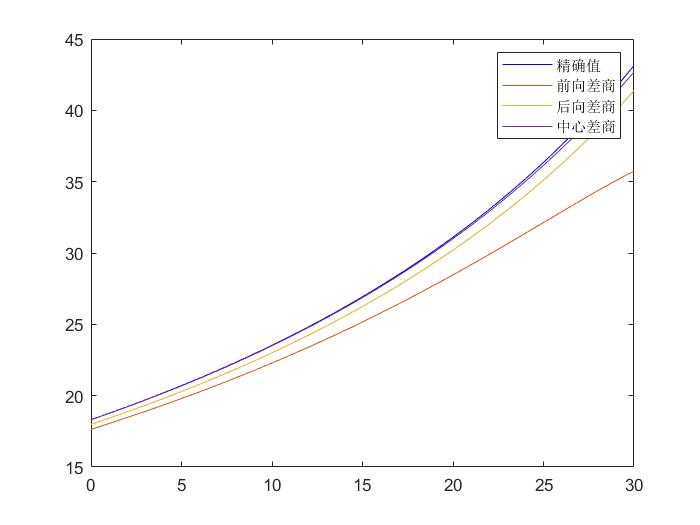
\includegraphics[width=10.5cm]{第五章作业/gaojingdu10.jpg}
    \caption{高精度微分公式(步长10)}
\end{figure}

\par
可以看出,步长较小时利用数值微分和使用解析法绘制出的加速度曲线基本相同。然而,当
步长取的较大时(这里以10为例),高精度微分公式的优势就明显体现出来了。并且在同一精度
的公式下, 中心差商的误差明显小于前向差商和后向差商。


\subsection{插值型数值微分}
\begin{figure}[H]
    \centering
    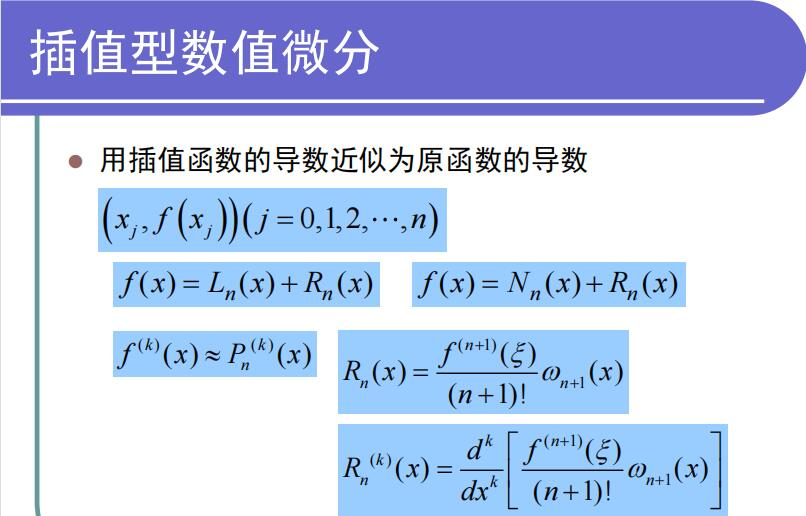
\includegraphics[width=14cm]{第五章作业/czwf.jpg}
\end{figure}
\begin{lstlisting}
%% Interpolation type numerical differentiation
clc,clear
step=1;
x0=0:step:30;
y0=v(x0);
% 三弯矩法方程组构造
for i=1:30/step
    h(i)=x0(i+1)-x0(i);
end
for i=1:30/step-1
    u(i)=h(i)/(h(i)+h(i+1));
    ld(i)=1-u(i);
    g(i)=6*((y0(i+2)-y0(i+1))/(x0(i+2)-x0(i+1))-(y0(i+1)-y0(i))/(x0(i+1)-x0(i)))/(h(i)+h(i+1));
end
A=zeros(30/step+1,30/step+1);
b=zeros(30/step+1,1);
A(1,1)=2;A(1,2)=1;
for i=2:30/step
    A(i,i-1)=u(i-1);A(i,i)=2;A(i,i+1)=ld(i-1);
end
A(30/step+1,30/step)=1;
A(30/step+1,30/step+1)=2;
b(1)=6*((y0(2)-y0(1))/(x0(2)-x0(1))-0)/h(1);
for i=2:30/step
    b(i)=g(i-1);
end
b(30/step+1)=6*(0-(y0(30/step+1)-y0(30/step))/(x0(30/step+1)-x0(30/step)))/h(30/step);
X=A\b;
% 绘图
step0=1e-5;
x=0:step0:30-step0;
count=1;
for t=0:step0:30-step0
    i=floor(t/step)+1;
    y(count)=1/(6*h(i))*(X(i)*(x0(i+1)-t)^3+X(i+1)*(t-x0(i))^3)+(y0(i)-X(i)*h(i)^2/6)*(x0(i+1)-t)/h(i)+(y0(i+1)-X(i+1)*h(i)^2/6)*(t-x0(i))/h(i);
    dy(count)=1/(6*h(i))*(X(i)*3*(x0(i+1)-t)^2*(-1)+X(i+1)*3*(t-x0(i))^2)+(y0(i)-X(i)*h(i)^2/6)*(-1)/h(i)+(y0(i+1)-X(i+1)*h(i)^2/6)*(1)/h(i);
    dv(count)=1800/(64-t)-9.8;
    count=count+1;
end
plot(x0,y0,'o');
hold on;
plot(x,y);

subplot(2,1,1)
plot(x,dv,'r')
subplot(2,1,2)
plot(x,dy,'b')
\end{lstlisting}
\begin{figure}[H]
    \centering
    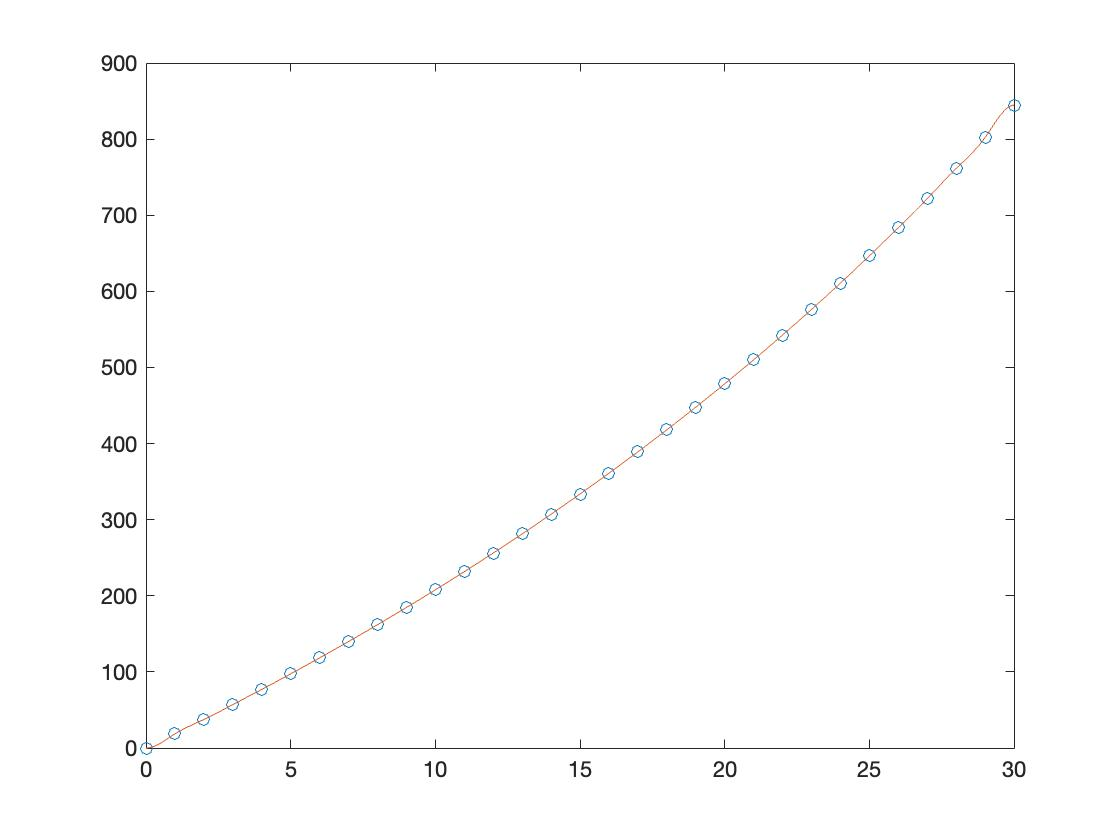
\includegraphics[width=10.5cm]{第五章作业/sanciyangtiao.jpg}
    \caption{三次样条插值结果}
\end{figure}
\begin{figure}[H]
    \centering
    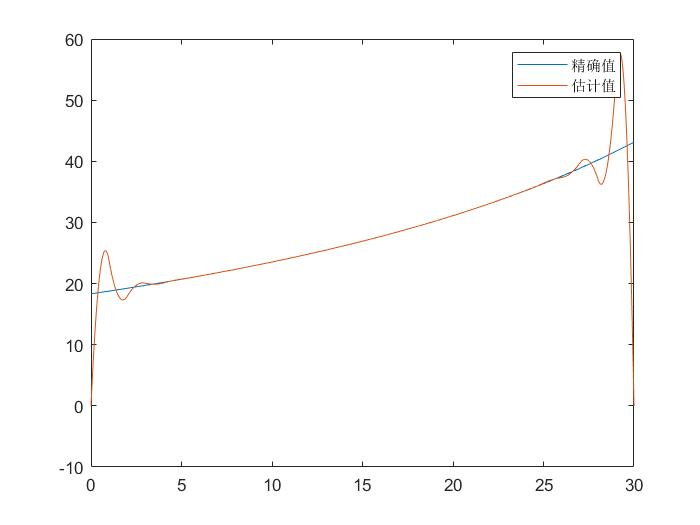
\includegraphics[width=10.5cm]{第五章作业/chazhiweifen.jpg}
    \caption{利用三次样条插值估计微分的结果}
\end{figure}

可以看出,在中间部分用插值函数的导数来近似求原函数微分效果相当好,然而在一头一尾
会出现类似龙格现象,并且边界条件确定也存在问题问题,求得的微分值偏差较大。


\section{小结}
本文从火箭发射过程的速度公式出发,分别使用数值积分和数值微分方法
得到了火箭发射过程中的高度和加速度与时间的关系。本文对数值积分各种方法
的优劣程度进行了讨论,并且分析、估计了相应的误差;同时,本文使用多种方法
利用数值微分方法画出了加速度与时间的关系图,取得了良好的效果。

\end{document}